\documentclass[11pt]{scrartcl}
\usepackage[sexy]{evan}

\usepackage{answers}
\Newassociation{hint}{hintitem}{all-hints}
\renewcommand{\solutionextension}{out}
\renewenvironment{hintitem}[1]{\item[\bfseries #1.]}{}

\usepackage{venndiagram,multicol}

\begin{document}
\title{Lógica}
\author{Ricardo Largaespada}
\date{03 Febrero 2024}

\maketitle

\section{Introducción}

Cuando leemos un problema de matemática, inmediatamente podemos ver que está dividido en dos partes: la información y las preguntas. Aprenderás, durante tu jornada como olímpico, que para resolver un problema de matemática, debes conocer varias técnicas. Una de las más básicas es saber organizar la información que se ofrece en los problemas.

\section{Problemas Resueltos}
\begin{example}
La investigación realizada con los niños de la ASJTNic, que recopiló las preferencias en cuanto a tres juegos: Ajedrez (designado por A), Bingo (designado por B) y Crucigrama (designado por C), indicó los siguientes resultados:
\begin{center}
\begin{tabular}{|c|c|c|c|c|c|c|c|c|}
\hline
Juegos & A & B & C & A y B & A y C & B y C & A, B y C & Ninguno \\
\hline
Preferencia & 100 & 150 & 200 & 20 & 30 & 40 & 10 & 130 \\
\hline
\end{tabular}
\end{center}
\begin{enumerate}
    \item[(a)] ¿Cuántos niños fueron consultados?
    \item[(b)] ¿Cuántos niños aprecian solo un juego?
    \item[(c)] ¿Cuántos niños aprecian más de un juego?
\end{enumerate}
\end{example}

Debes haber notado que hay una gran cantidad de información proporcionada. De alguna manera, esta información ya está organizada en una tabla. Pero para resolver el problema, cambiaremos nuestra representación, nuestro punto de vista. Vamos a construir un diagrama de Venn, el popular diagrama de conjuntos:
\begin{center}
\begin{venndiagram3sets}[labelOnlyA={60},labelOnlyB={100},labelOnlyC={140},
labelOnlyAB={10},labelOnlyAC={20},labelOnlyBC={30},labelABC={10},
labelNotABC={130}]
\end{venndiagram3sets}
\end{center}

Ahora podemos responder a las preguntas fácilmente:
\begin{enumerate}
    \item[(a)] Fueron consultados \(10 + 10 + 20 + 30 + 60 + 100 + 140 + 130 = 500\) niños.
    \item[(b)] \(60 + 100 + 140 = 300\) niños les gusta solo un juego.
    \item[(c)] \(10 + 10 + 20 + 30 = 70\) niños aprecian más de un juego.
\end{enumerate}

\begin{example}
Carlitos posee seis monedas, siendo una de ellas falsa. Desconocemos el peso de una moneda falsa y tampoco sabemos el peso de una moneda verdadera; únicamente tenemos la certeza de que las monedas verdaderas tienen todas el mismo peso, mientras que la moneda falsa tiene un peso diferente. Contamos con una balanza de dos platillos. Muestra cómo es posible descubrir la moneda falsa utilizando tan solo tres pesajes.
\end{example}

Sean A, B, C, D, E y F las monedas. En primer lugar, realizamos el pesaje
\( (AB) \; <> \; (CD) \) (lo que significa que A y B están en un platillo y C y D en el otro). Si \( (AB) = (CD) \) (es decir, si está equilibrado), entonces E o F son falsas. En este caso, realizamos el pesaje \( (A) \; <> \; (E) \). Si está equilibrado, F es falsa. De lo contrario, E es falsa.

Ahora, si no hubo equilibrio en \( (AB) \; <> \; (CD) \), entonces E y F son verdaderas. Luego, realizamos el pesaje \( (AB) \; <> \; (EF) \). Si está equilibrado, entonces C o D son falsas. En este caso, realizamos el pesaje \( (A) \; <> \; (C) \). Si está equilibrado, D es falsa. De lo contrario, C es falsa.

Para finalizar, si \( (AB) <> (EF) \), entonces A o B es falsa. En este caso, realizamos el pesaje \( (A) \; <> \; (C) \). Si está equilibrado, B es falsa. De lo contrario, A es falsa.

Continuando con el proceso de desarrollo del razonamiento, resolveremos a continuación dos preguntas relacionadas con la siguiente pregunta: ¿Será posible?. A lo largo del año, verás cómo esta pregunta es frecuente en la olimpiada. De hecho, es recurrente en toda la matemática. Aquí también desarrollaremos una de las técnicas más poderosas utilizadas para resolver problemas de matemática, que es la idea de la prueba por absurdo.

\begin{example}
¿Es posible cortar un rectángulo de \(5 \times 6\) en ocho rectángulos diferentes con dimensiones enteras y lados paralelos a los lados del rectángulo mayor?\end{example}

Supongamos que todos los rectángulos son distintos. Los rectángulos con el área más pequeña posible son:
\begin{multicols}{2}
\begin{enumerate}
    \item Área 1: $1 \times 1$
    \item Área 4: $2 \times 2$ y $1 \times 4$
    \item Área 2: $1 \times 2$
    \item Área 5: $1 \times 5$
    \item Área 3: $1 \times 3$
    \item Área 6: $2 \times 3$ y $1 \times 6$
\end{enumerate}
\end{multicols}

Obsérvese que la menor superficie cubierta por ocho rectángulos distintos debe ser al menos \(1 + 2 + 3 + 4 + 4 + 5 + 6 + 6 = 31 > 30\). Por tanto, es imposible obtener 8 rectángulos distintos.\\

Es importante tener cuidado con este tipo de afirmaciones porque, en algunos casos, es
posible.

\begin{example}
Podemos intercambiar un entero positivo \( n \) por el producto \( a \times b \) donde \( a \) y \( b \) son enteros positivos tales que \( a + b = n \). ¿Podemos obtener 2024 a partir de 22 mediante una secuencia de intercambios?
\end{example}

Note que \(2024 = 44 \times 46\) puede ser obtenido de \(44 + 46 = 90\), que puede ser obtenido de \(15 + 6 = 21\). Por otro lado, cualquier número \( n - 1 = (n - 1) \times 1 \)
puede ser obtenido de \( (n - 1) + 1 = n \). Así, basta seguir la secuencia siguiente:
\[ 22 \rightarrow 21 \rightarrow 90 \rightarrow 2024 \]

\Opensolutionfile{all-hints}

\section{Problemas Propuestos}
\begin{problem}
    Le dan 4 monedas aparentemente idénticas. Se sabe que una de ellas es falsa (tiene un peso diferente a las demás y no se sabe si es más ligera o más pesada). Muestre cómo encontrar la moneda falsa pesándola dos veces en una balanza de dos platillos.
    \begin{hint}
    Puedes pesar monedas ya pesadas.
        \begin{center}
        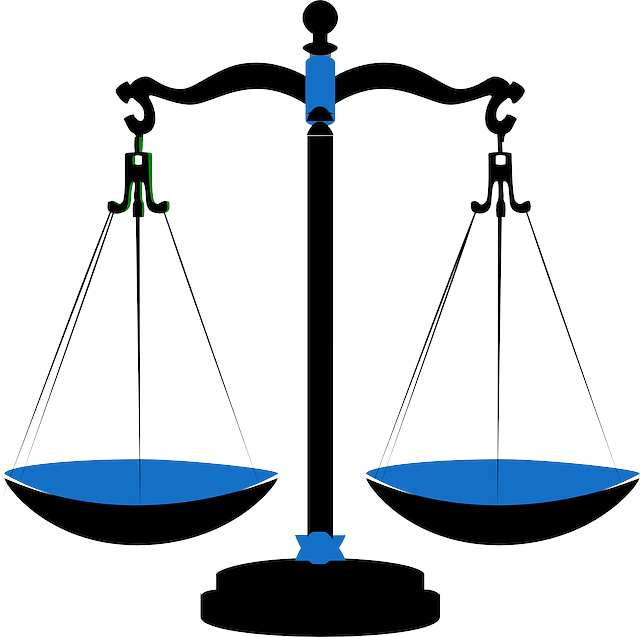
\includegraphics[scale=0.5]{clase_02_Algoritmos_balanzas.jpg}
        \end{center}
    \end{hint}
\end{problem}

\begin{problem}\label{p3.2}
    Una de las nueve monedas es falsa, pesa menos que una moneda real. ¿Cómo determinar la moneda falsa en 2 pesadas?
    \begin{hint}
        Dividir el conjunto de monedas sospechosas en tres partes iguales por cada pesada; luego, para cualquier resultado, el número de monedas sospechosas se reduce exactamente a la tercera parte.
    \end{hint}
\end{problem}

\begin{problem}
Una de las 27 monedas es falsa, pesa menos que una real.
\begin{itemize}
\item[a)] ¿Cómo determinar la moneda falsa en 3 pesadas?
\item[b)] Resuelve el mismo problema para 26 monedas.
\item[c)] Piense cómo generalizar la solución a cualquier número de monedas de 10 a 27.
\end{itemize}
    \begin{hint}
        Puedes intentar reducir al problema \eqref{p3.2}.
\begin{comment}
(a) Colocamos 9 monedas en cada platillo. Para cualquier resultado de esta pesada, quedar´an
9 monedas sospechosas, y tendremos dos pesadas m´as a nuestra disposici´on. Esto ya lo
podemos resolver debido al problema 1
(b) Colocamos 9 monedas en cada platillo. En el caso del desequilibrio (que uno de los platillos
pese m´as que el otro), llegamos al problema 1 y, en el caso del equilibrio, solo quedan ocho
monedas sospechosas (las 18 colocadas en los platillos necesariamente son reales). A˜nadimos
cualquiera de las 18 monedas utilizadas en la primera pesada, y de nuevo reducimos
el problema al ya resuelto (el problema 1).
(c) Suponga que hay N monedas en total. Colocamos N
3  en cada platillo, reserve las restantes.
Si uno de los platillos pes´o m´as, entonces quedan N
3  monedas sospechosas, y en
el caso de equilibrio, quedan N − 2 N
3  monedas sospechosas. Dado que todas las dem´as
monedas deben ser reales, y el n´umero total de monedas es al menos diez, el conjunto de
monedas sospechosas puede complementarse con monedas reales hasta nueve y as´ı llegamos
al problema 1.
\end{comment}
\end{hint}
\end{problem}

\begin{problem}
    Demuestra que es posible ordenar los números del 1 al 16 de forma que la suma de dos números vecinos sea siempre un número cuadrado perfecto.
\end{problem}

\begin{problem}
    Víctor y María empiezan a trabajar el mismo día. Víctor trabaja 3 días seguidos y luego tiene un día de descanso. María trabaja 7 días seguidos y descansa los otros 3. ¿Cuántos días de descanso tuvieron en común los dos durante los primeros 1000 días?
    \begin{hint}
        Encuentra un ciclo de tamaño 20.
    \end{hint}
\end{problem}

\begin{problem}
    Como recortar un rectángulo \(3 \times 13\) en trece rectángulos menores distintos?
    \begin{hint}
Encuentra los rectángulos con área mínima.
    \end{hint}
\end{problem}

\begin{problem}[Olimpiada de Mayo]
En un año con 53 sábados, ¿qué día de la semana es el 12 de mayo? ¿Mayo? Nombra todas las posibilidades.
    \begin{hint}
        Considere que \(365=52\times 7+1\).
    \end{hint}
\end{problem}

\begin{problem}[Bulgaria]
    Evan escribe todos los números enteros del 1 al 100 (ambos inclusive) en tarjetas y le da algunas de ellas a Elisa. Se sabe que para dos cualesquiera de estas tarjetas, una de Evan y otra de Elisa, la suma de los números no está con Evan y el producto no está con Elisa. Determina el número de cartas de Elisa, sabiendo que la carta 13 la tiene Evan.
\end{problem}

\begin{problem}[Rusia]
Demuestre que los números del 1 al 15 no pueden dividirse en un grupo A de dos elementos y un grupo B de 13 elementos tal que la suma de los elementos de B sea igual al producto de los elementos de A.
\end{problem}

\begin{problem}
Escribimos un número entero en cada cuadrado de un tablero de 8 veces 8. Se sabe que para cada casilla, la suma de sus vecinas es 1. Halla la suma de todos los números del tablero.
Nota: Consideramos que los cuadrados vecinos tienen un lado en común.
\end{problem}

\begin{problem}
Eduardo pensó en cinco números diferentes y escribió en la pizarra los diez números que son la suma de dos de estos cinco números. ¿Puede Orlando averiguar los números en los que pensó Eduardo con sólo mirar los números escritos en la pizarra?
\end{problem}

\Closesolutionfile{all-hints}

\section{Sugerencias}
\begin{enumerate}
\input{all-hints.out}
\end{enumerate}

\end{document}